%!TEX root = ../thesis.tex

\chapter{Introduction}
\label{chap:introduction}
Since the middle of the 20th century humanity has sent spacecraft to every planet in our solar system at least once. These probes have given us a wealth of information about these planets, their history and evolution. Unfortunately the information returned to us is somewhat biased towards the surface of these planets. This ignorance speaks to the difficulty of observing the interiors of planets. Even our knowledge of our own planet, which is readily accessible to observation, becomes much murkier as we delve deeper. 

Fortunately on many planets there is a way to make direct observations of the processes occurring in the deepest layers of planets: by observing planetary magnetic fields. Planetary magnetic fields are generated by a process called a planetary dynamo \citep{larmor1919, jones2011}. In a dynamo the complex motion of electrically conducting fluids generates a magnetic field that can be observed on the surface, or in orbit. Furthermore, these planetary magnetic fields are keenly sensitive to their environment and display a wide range of strengths, and morphologies \citep{connerney2007, christensen2009review}.

Even the existence of a planetary magnetic field tells us much about the deep interior of a planet. For example it tells us that there is an electrically conducting fluid in the deep interior. It also indicates that this fluid may be convecting, providing an energy source for the dynamo. For example, if natural convection is responsible for the fluid motion, this implies a minimum heat flux out of the core which reveals information concerning the state of the shallower planetary interior (e.g. the vigour of mantle convection) \citep{breuer2010}.

Planetary magnetic fields also vary in time as the fluid that generates them flows and convects. Each magnetic field line can be directly connected to a parcel of fluid in the core, so the short-timescale variation of the field can be used to derive the flows at the top of the core \citep{bloxham1991,finlay2003}.

Finally, planetary magnetic fields have morphologies that differ depending on their geological context. These wildly differing morphologies can provide excellent tests for theories of planetary composition, high pressure mineralogy and the thermal evolution of planets \citep{stevenson2003}.

Our solar system displays a great diversity of planetary magnetic fields \citep{connerney2007}. Some planets have no active dynamo; we have no evidence of active dynamos on Venus \citep{smith1963, smith1965} and only crustal magnetism from a past active dynamo on Mars \citep{acuna1999}. Other planets have predominantly dipolar magnetic fields (Mercury \citep{anderson2012}, Earth \citep{igrf11}, Jupiter \citep{connerney1992}, and Saturn \citep{cao2011}: figures \ref{fig:Mercurybrintro}, \ref{fig:Earthbr}, \ref{fig:Jupiterbr}, \ref{fig:Saturnbr} respectively), though each of these presents their own mysteries \citep{stevenson2003}. Finally Uranus (figure \ref{fig:Uranusbr}) and Neptune (figure \ref{fig:Neptunebr}) have very non-dipolar planetary magnetic fields \citep{holme1996}.  
\begin{figure}
	\centering
	 \begin{subfigure}[b]{0.47\textwidth}
                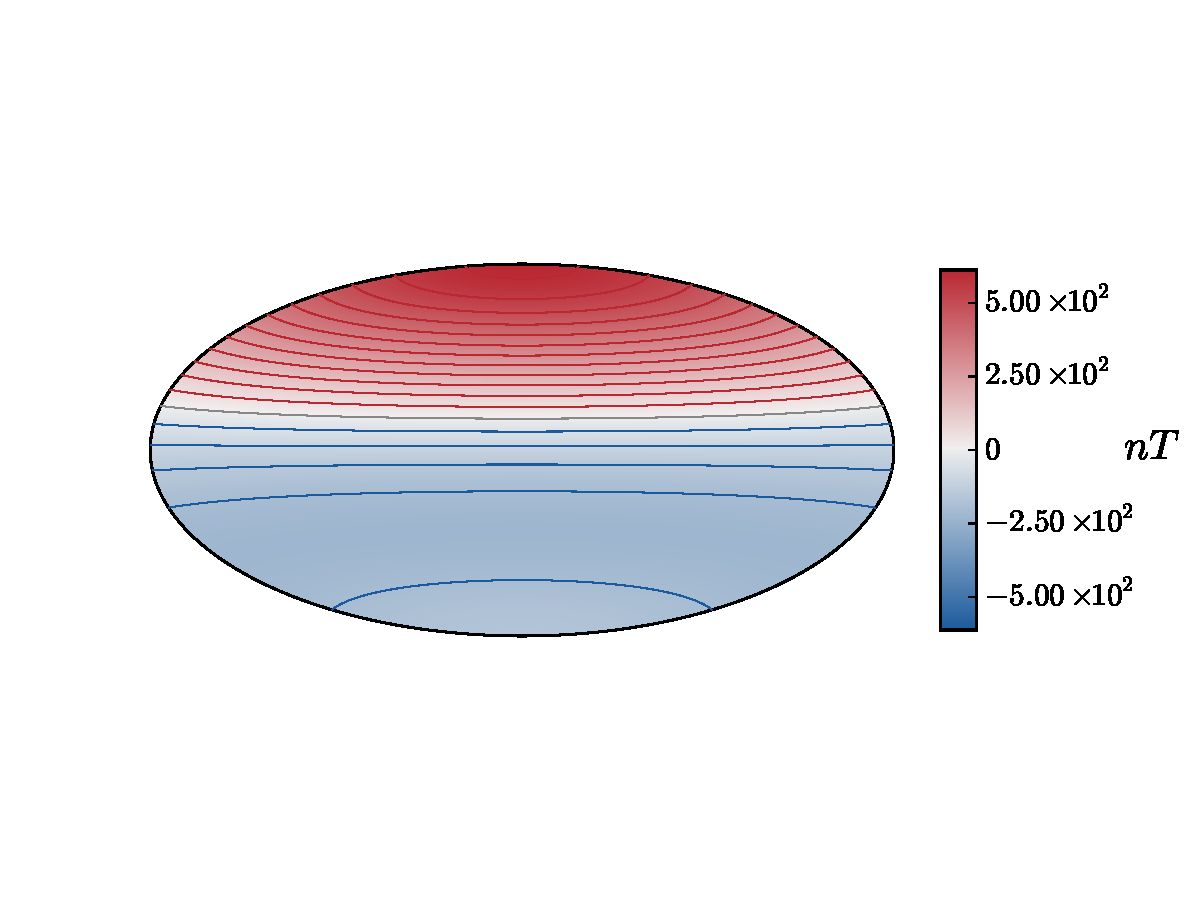
\includegraphics[width=\textwidth]{Chapter1/Figures/Mercury.pdf}
                \caption{Mercury \citep{anderson2012}}
                \label{fig:Mercurybrintro}
        \end{subfigure}
        	 \begin{subfigure}[b]{0.47\textwidth}
                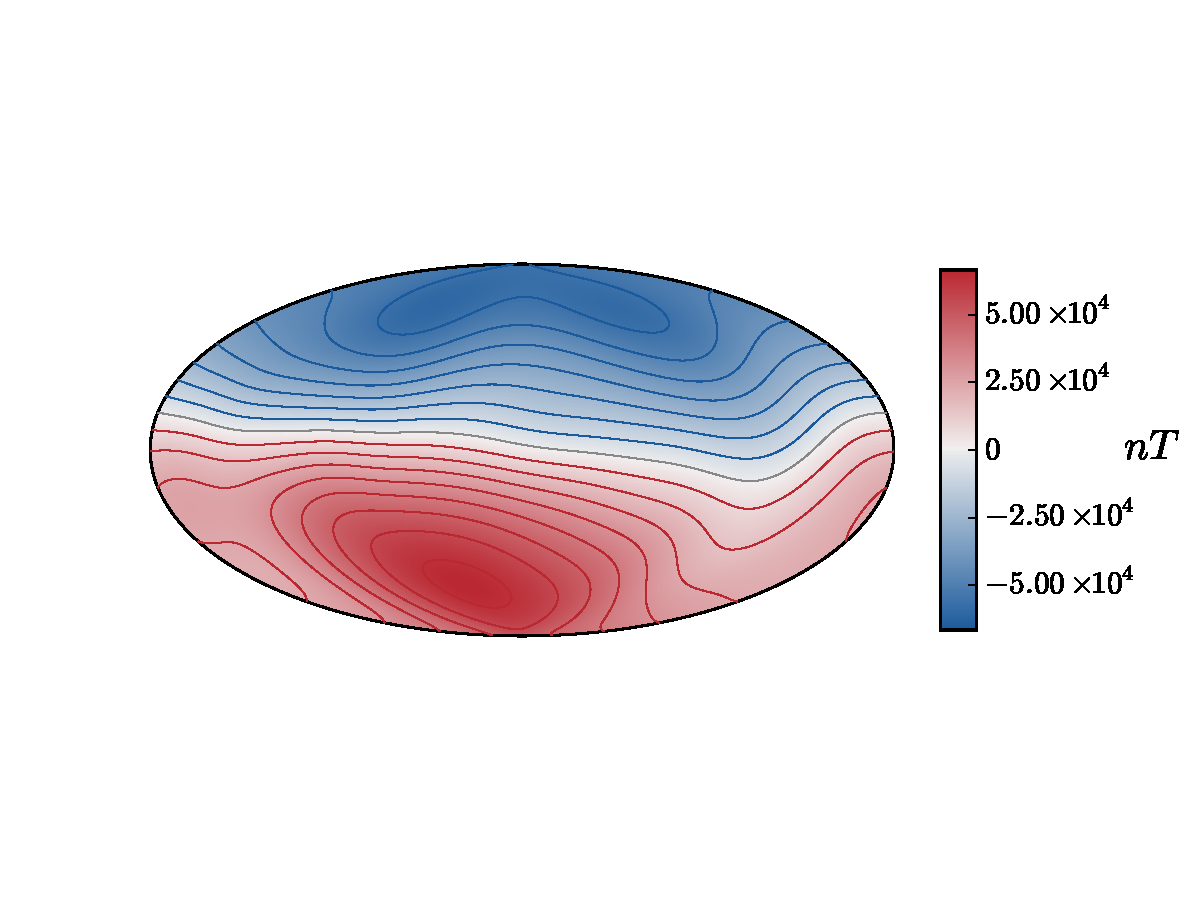
\includegraphics[width=\textwidth]{Chapter1/Figures/Earth.pdf}
                \caption{Earth \citep{igrf11}}
                \label{fig:Earthbr}
        \end{subfigure}
        	\begin{subfigure}[b]{0.47\textwidth}
                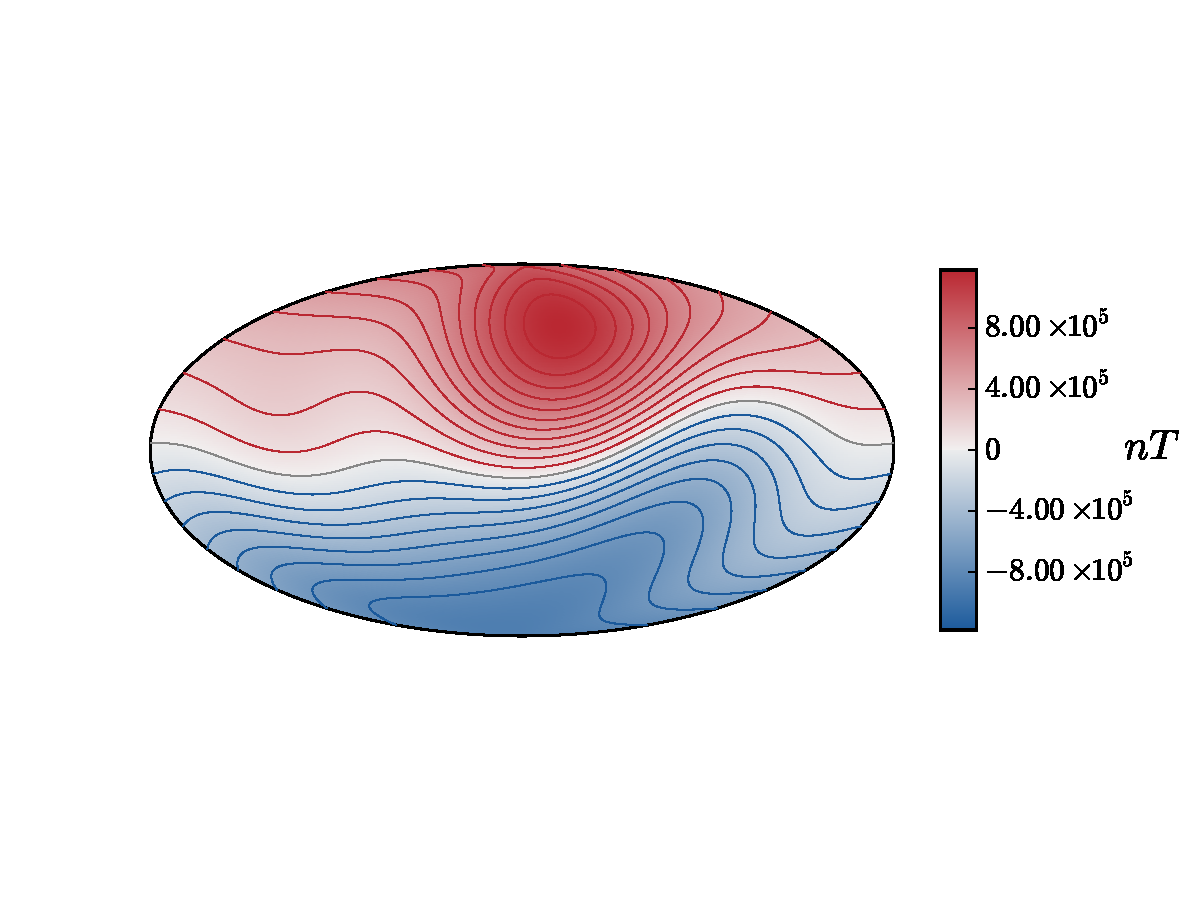
\includegraphics[width=\textwidth]{Chapter1/Figures/Jupiter.pdf}
                \caption{Jupiter \citep{connerney1992}}
                \label{fig:Jupiterbr}
        \end{subfigure}
        	\begin{subfigure}[b]{0.47\textwidth}
                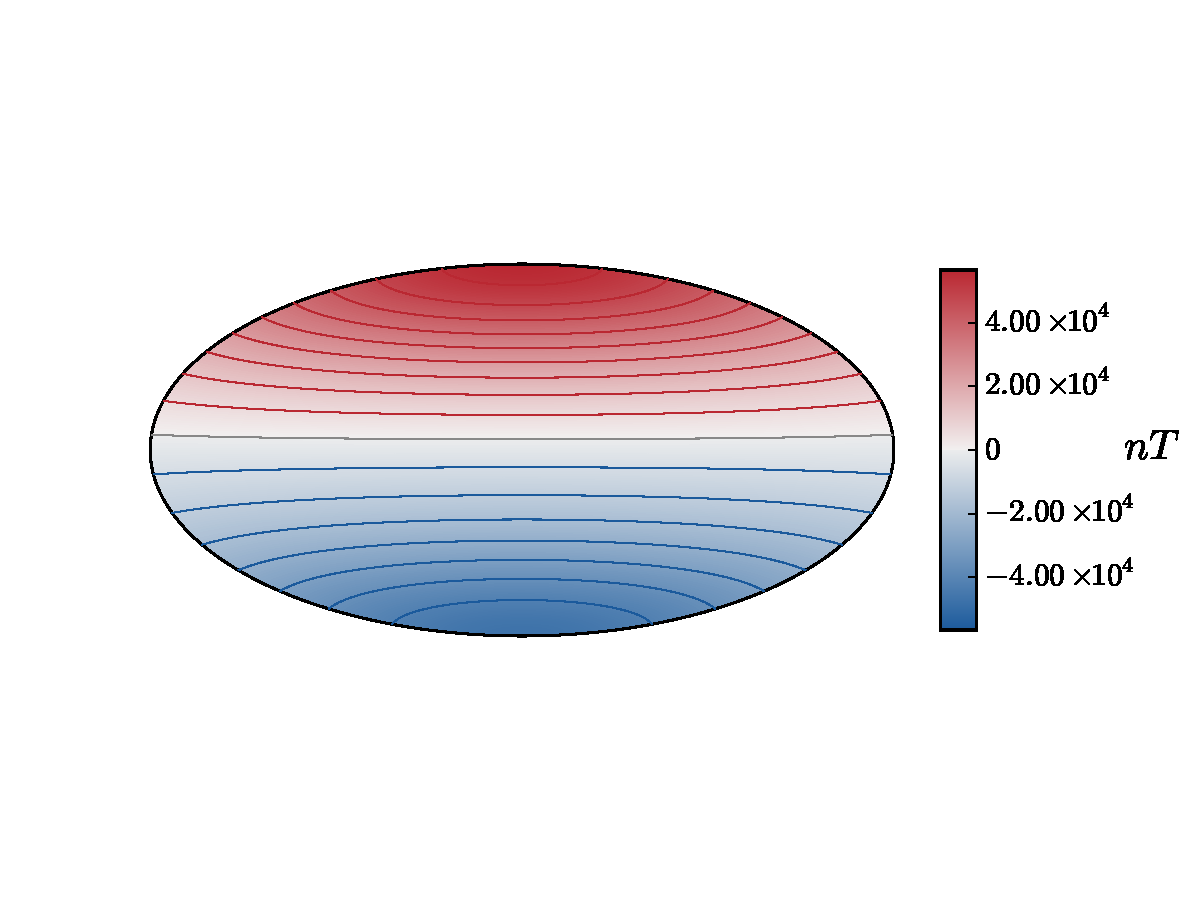
\includegraphics[width=\textwidth]{Chapter1/Figures/Saturn.pdf}
		\caption{Saturn \citep{cao2011}}
                \label{fig:Saturnbr}
        \end{subfigure}
        	\begin{subfigure}[b]{0.47\textwidth}
                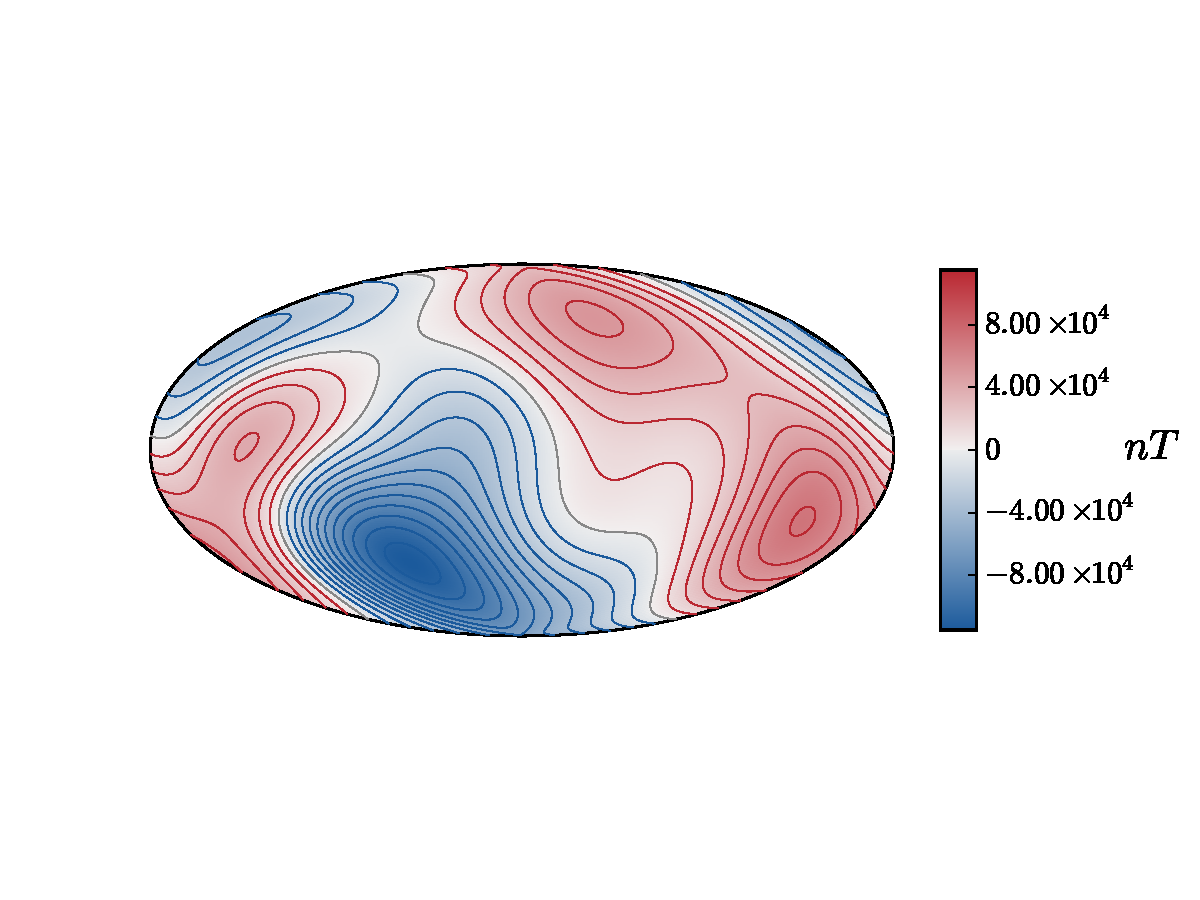
\includegraphics[width=\textwidth]{Chapter1/Figures/Uranus.pdf}
                \caption{Uranus \citep{holme1996}}
                \label{fig:Uranusbr}
        \end{subfigure}
        	\begin{subfigure}[b]{0.47\textwidth}
                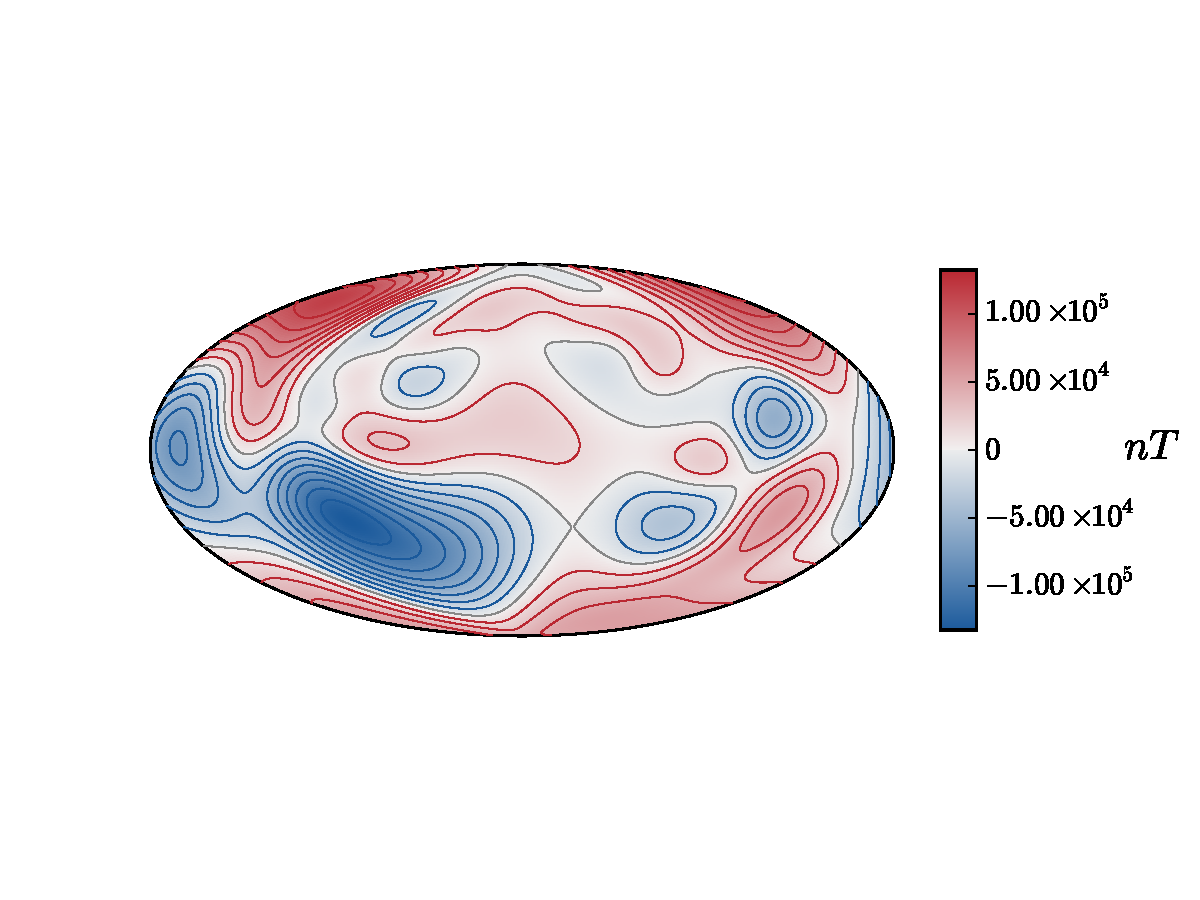
\includegraphics[width=\textwidth]{Chapter1/Figures/Neptune.pdf}
                \caption{Neptune \citep{holme1996}}
                \label{fig:Neptunebr}
        \end{subfigure}
        \caption{The radial magnetic field for each planet in our solar system at the planetary surface.}
\end{figure}

This wide range of planetary magnetic field morphologies generated by active dynamos indicates several important concepts about planetary magnetic fields. First, it shows that dynamos are very sensitive to the geophysical context in which they find themselves. The most striking example of this is the difference between Venus and Earth. Despite the many similarities between these planets (size and composition being foremost among them), Earth has possessed an active dynamo for at least 3.4 billion years \citep{tarduno2010} whereas we have no evidence that Venus ever possessed an active dynamo \citep{russell1980}. Conversely, Jupiter and Earth are dissimilar by most metrics, yet both generate predominantly dipolar magnetic fields that are morphologically similar (Figures \ref{fig:Earthbr} and \ref{fig:Jupiterbr}). 

Secondly, this diversity shows that there are many different ``types'' of planetary magnetic fields which share a common mechanism of generation. It is not unreasonable to assume that there are even more classes of dynamos which are not represented in our solar system, because of the small number of planets this system possesses.

In the last decade, ground based observations and the Kepler spacecraft have found hundreds of exoplanets around other stars \citep{rein2015}. These newly discovered planets possess a range of physical properties (e.g. pressures, temperatures \citep{seager2007, valencia2006}, and  compositions \citep{elkins2008, elkins2008coreless}) that are much more diverse and extreme than the physical properties of the planets within our solar system. This naturally raises the question of how the exotic physical properties of exoplanets could affect the existence, detectability and morphology of the dynamos they may possess. 

Of particular interest is the class of terrestrial planets with a mass greater than that of Earth, ``super-Earth's''. These planets are interesting because the pressures and temperatures which must exist in them are not found in any terrestrial body in our solar system. These extreme pressures mean that the constituent materials can behave much differently than they do at the lower pressures within the terrestrial planets of our own solar system \citep{karato2011}. 

This work will focus on testing the effects of novel material properties and solidification regimes on magnetic field generation. First we focus on two ways of reproducing the anomalously weak magnetic field observed at the planet Mercury. These mechanisms use results from high pressure mineralogy and from gravity surveys of Mercury from the recent MESSENGER spacecraft. In the second part we use results from theoretical and experimental high pressure mineralogy to predict the effect of mantle metallization on exoplanetary magnetic fields. 